\section{Radio Frequency Identification (RFID)}

	L'idea di RFID si è sviluppata come evoluzione elettronica dei codici a barre, per un'identificazione più rapida dei beni.
	
	La rete RFID si basa sulla presenza di due dispositivi di base: un lettore e un tag.
	Un lettore è composto da modulo a radiofrequenza (antenna), memoria, CPU, Batteria;
	un tag è composto da antenna, circuito di recupero dell'energia (trasmessa dal lettore), memoria non volatile per memorizzare l'ID, e in alcuni casi anche di sensori e una piccola CPU.
	Si distinguono 3 tipi di tag:
	\begin{description}
		\item[Passivi] Funzionano solo grazie al circuito di recupero dell'energia che cattura quella trasmessa dal lettore
		\item[Semi-passivi]  Dotati di batteria
		\item[Attivi] Dotati di batteria e trasmettitore
	\end{description}

	\paragraph{Electronic Product Code (EPC)}
	Ogni tag è dotato di un EPC, si tratta di uno standard che definisce un codice univoco del prodotto su 96 bit organizzati nel seguente modo:
	\begin{itemize}
		\item \textit{Header}. 8 bit, numero di versione del tag
		\item \textit{EPC Manager}. 28 bit, ID del produttore
		\item \textit{Object class}. 24 bit, ID del prodotto
		\item \textit{Serial number}. ID dell'unità
	\end{itemize}

	Le sfide nella realizzazione di un tag RFID sono la costruzione di un circuito di recupero dell'energia efficiente, la miniaturizzazione e il contenimento del costo.
	
	Le sfide nella realizzazione di un lettore RFID riguardano invece la realizzazione di antenne in grado di fornire sufficiente energia al tag, grande differenza nella magnitudo del segnale inviato e ricevuto e l'integrazione con i sistemi industriali più diffusi.
	
	\begin{figure}[h]
		\centering
		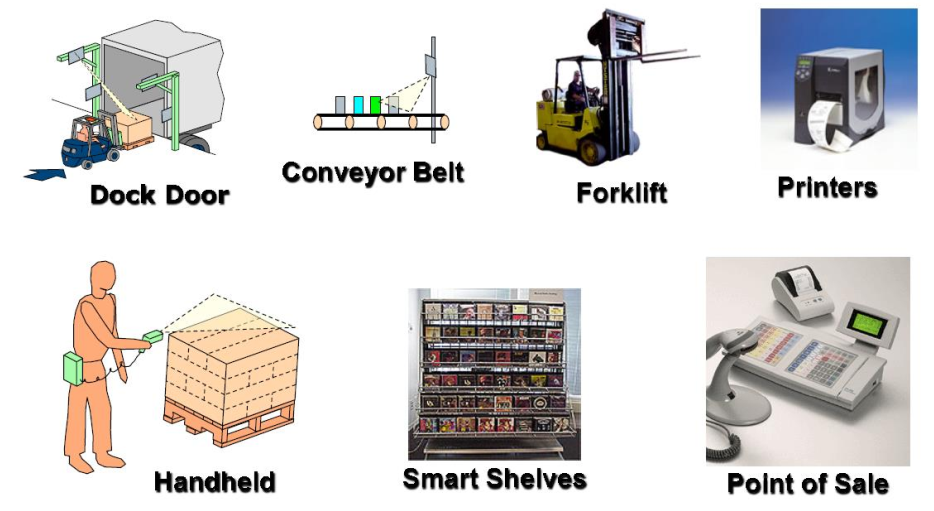
\includegraphics[width=0.8\textwidth]{lez7/useCasesRFID.png}
		\caption{Applicazioni reali che sfruttano RFID}
		\label{fig:useCasesRFID}
	\end{figure}

	RFID sfrutta le frequenze tra 100 e X MHz in quanto risultano essere quelle ottimali per la propagazione del segnale in ambienti affollati (Figura \ref{fig:frequenzaOttimale}).
	
	\begin{figure}[h]
		\centering
		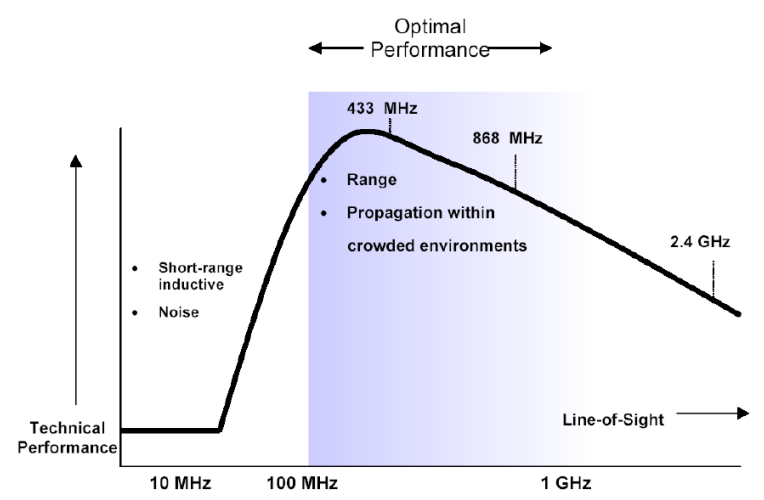
\includegraphics[width=0.6\textwidth]{lez7/optimalFrequency.png}
		\caption{Performance di trasmissione al variare della frequenza per RFID}
		\label{fig:frequenzaOttimale}
	\end{figure}


\section{Near Field Communication (NFC)}